\section{习题}

\begin{exercise}
求下列极限:
\begin{enumerate}
    \item $\underset{x\rightarrow -2}{\lim}\frac{x^2-x+2}{x^2+4}$
    \item $\underset{x\rightarrow 1}{\lim}\left( \frac{1}{1-x}-\frac{3}{1-x^2} \right) $
    \item $\underset{x\rightarrow 0}{\lim}\frac{\left| 2x-1 \right|-\left| 2x+1 \right|}{x}$
    \item $\underset{x\rightarrow 0}{\lim}\frac{x-\sin 2x}{x+\sin 5x}$
    \item $\underset{x\rightarrow \infty}{\lim}\left( \frac{x-4}{x+1} \right) ^{2x-1}$
    \item $\underset{x\rightarrow \infty}{\lim}\sin \left( 1+\frac{1}{x} \right) ^{2x+1}$
    \item $\underset{x\rightarrow \infty}{\lim}\lg \frac{100+x^2}{1+100x^2}$
\end{enumerate}
\end{exercise}

解:

1.
\[
\underset{x\rightarrow -2}{\lim}\frac{x^2-x+2}{x^2+4}=\left. \frac{x^2-x+2}{x^2+4} \right|_{x=-2}=1
\]

2.
\[
\underset{x\rightarrow 1}{\lim}\left( \frac{1}{1-x}-\frac{3}{1-x^2} \right) =\underset{x\rightarrow 1}{\lim}\frac{\left( x+2 \right) \left( x-1 \right)}{1-x^3}=-\underset{x\rightarrow 1}{\lim}\frac{x+2}{x^2+x+1}=-1
\]

3.
\[
\underset{x\rightarrow 0}{\lim}\frac{\left| 2x-1 \right|-\left| 2x+1 \right|}{x}=\underset{x\rightarrow 0}{\lim}\frac{\left( 1-2x \right) -\left( 2x+1 \right)}{x}=\underset{x\rightarrow 0}{\lim}\frac{-4x}{x}=-4
\]

4.
\[
\underset{x\rightarrow 0}{\lim}\frac{x-\sin 2x}{x+\sin 5x}=\underset{x\rightarrow 0}{\lim}\frac{1-2\frac{\sin 2x}{2x}}{1+5\frac{\sin 5x}{5x}}=-\frac{1}{6}
\]

5.
\begin{align*}
&\underset{x\rightarrow \infty}{\lim}\left( \frac{x-4}{x+1} \right) ^{2x-1}=\underset{x\rightarrow \infty}{\lim}\left( 1+\frac{-5}{x+1} \right) ^{2\left( x+1 \right) -3} \\
&=\underset{x\rightarrow \infty}{\lim}\left( 1+\frac{-10}{2\left( x+1 \right)} \right) ^{2\left( x+1 \right)}\cdot \underset{x\rightarrow \infty}{\lim}\left( 1-10\frac{1}{2\left( x+1 \right)} \right) ^{-3} \\
&=\underset{t\rightarrow \infty}{\lim}\left( 1+\frac{-10}{t} \right) ^t\cdot 1^{-3}=e^{-10}
\end{align*}

6.
\begin{align*}
&\underset{x\rightarrow \infty}{\lim}\sin \left[ \left( 1+\frac{1}{x} \right) ^{2x+1} \right] =\sin \underset{x\rightarrow \infty}{\lim}\left( 1+\frac{2}{2x} \right) ^{2x+1} \\
&=\sin \left[ \underset{x\rightarrow \infty}{\lim}\left( 1+\frac{2}{2x} \right) ^{2x}\cdot \underset{x\rightarrow \infty}{\lim}\left( 1+\frac{2}{2x} \right) ^1 \right] =\sin \left( e^2\cdot 1 \right)
\end{align*}

7.
\[
\underset{x\rightarrow \infty}{\lim}\lg \frac{100+x^2}{1+100x^2}=\lg \underset{x\rightarrow \infty}{\lim}\frac{100+x^2}{1+100x^2}=\lg \frac{1}{100}=-2
\]

\begin{tcolorbox}
本题还是以直接带入为主,有些小题需要化简一下式子而已。
\end{tcolorbox}

~

\begin{exercise}
求$\underset{x\rightarrow +\infty}{\lim}\left( \sin \sqrt{x+1}-\sin \sqrt{x} \right) $。
\end{exercise}

解:

总体思路是将两个三角函数合并到一个,然后考察三角函数内多项式的极限。

首先化简三角函数:
\[
\underset{x\rightarrow +\infty}{\lim}\left( \sin \sqrt{x+1}-\sin \sqrt{x} \right) =\underset{x\rightarrow +\infty}{\lim}2\cos \frac{\sqrt{x+1}+\sqrt{x}}{2}\sin \frac{\sqrt{x+1}-\sqrt{x}}{2}
\]
然后考察$\cos \frac{\sqrt{x+1}+\sqrt{x}}{2}$,是有界函数,再考察$\sin \frac{\sqrt{x+1}-\sqrt{x}}{2}$,当$x\rightarrow \infty $时似乎$\sqrt{x+1}-\sqrt{x}\rightarrow 0$:
\begin{align*}
&\because \frac{\sqrt{x+1}-\sqrt{x}}{2}=\frac{1}{2\left( \sqrt{x+1}+\sqrt{x} \right)} \\
&\therefore \underset{x\rightarrow +\infty}{\lim}\sin \frac{\sqrt{x+1}-\sqrt{x}}{2}=\sin \underset{x\rightarrow +\infty}{\lim}\frac{1}{2\left( \sqrt{x+1}+\sqrt{x} \right)}=\sin 0=0
\end{align*}
所以:
\[
\underset{x\rightarrow +\infty}{\lim}\left( \sin \sqrt{x+1}-\sin \sqrt{x} \right) =\underset{x\rightarrow +\infty}{\lim}\left( 2\cos \frac{\sqrt{x+1}+\sqrt{x}}{2}\cdot 0 \right) =0
\]

~

\begin{exercise}
若
\[
\begin{cases}
	\underset{x\rightarrow a}{\lim}\left[ f\left( x \right) +g\left( x \right) \right] =2\\
	\underset{x\rightarrow a}{\lim}\left[ f\left( x \right) -g\left( x \right) \right] =1\\
\end{cases}
\]
求$\underset{x\rightarrow a}{\lim}\left[ f\left( x \right) \cdot g\left( x \right) \right] $。
\end{exercise}

解:

总体思路是采用极限的线性组合。
\begin{align*}
&\because \begin{cases}
	\underset{x\rightarrow a}{\lim}\left[ f+g \right] ^2=\underset{x\rightarrow a}{\lim}\left[ f^2+g^2+2fg \right] =4\\
	\underset{x\rightarrow a}{\lim}\left[ f-g \right] ^2=\underset{x\rightarrow a}{\lim}\left[ f^2+g^2-2fg \right] =1\\
\end{cases} \\
&\therefore \underset{x\rightarrow a}{\lim}fg=\frac{1}{4}\left( 4-1 \right) =\frac{3}{4}
\end{align*}

~

\begin{exercise}
若有方程$x^3-3x=1$,讨论其在$\left[ 1,2 \right] $上有无根。
\end{exercise}

解:

总体思路是考察连续函数的根存在定理。

令$y=x^3-3x-1$,则$y$在$\left[ 1,2 \right] $上连续,且:
\[
y\left( 1 \right) \cdot y\left( 2 \right) =-3<0
\]
根据根存在定理,必有根。

~

\begin{exercise}
如下图,等边三角形内放置直径相同的若干个圆,图示为10个,三角形外切圆。当增大圆的个数时,能否覆盖三角形,如能则最终需要多少个,如不能,则最终能覆盖多少三角形面积。
\begin{figure}[h]
\centering
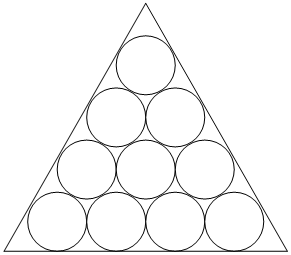
\includegraphics[height=2.5cm]{1.3.png}
\end{figure}
\end{exercise}

解:

总体思路是考察圆的总面积和三角形面积的比例的极限。

假设三角形面积$A$,所有圆面积之和$A_n$,圆半径$r$,一边放$n$个,一共$\frac{1}{2}n\left( n-1 \right) $个圆。于是所有圆面积之和$A_n$为:
\[
A_n=\pi r^2\cdot \frac{1}{2}n\left( n+1 \right)
\]
易得三角形边长$L=2\left( n-1 \right) r+2\sqrt{3}\cdot r$,于是三角形面积$A$为:
\[
A=\frac{1}{2}\cdot L\cdot \frac{\sqrt{3}}{2}L=\frac{\sqrt{3}}{4}\left[ 2\left( n-1 \right) r+2\sqrt{3}r \right] ^2
\]
于是:
\[
\underset{n\rightarrow \infty}{\lim}\frac{A_n}{A}=\underset{n\rightarrow \infty}{\lim}\frac{\pi r^2\cdot \frac{1}{2}n\left( n+1 \right)}{\frac{\sqrt{3}}{4}\left[ 2\left( n-1 \right) r+2\sqrt{3}r \right] ^2}=\frac{\pi r^2\cdot \frac{1}{2}}{\frac{\sqrt{3}}{4}\cdot 4r^2}=\frac{\pi}{2\sqrt{3}}=0.9069
\]
最多只能覆盖三角形的90\%多一点的面积。




